% Created 2026-04-21 Tue 19:39
% Intended LaTeX compiler: lualatex
\DocumentMetadata{lang = en, pdfversion = 2.0, pdfstandard = ua-2, pdfstandard = a-4, testphase = {phase-III, title, table, math, firstaid}}
\documentclass[11pt]{article}
\usepackage{amsmath}
\usepackage{fontspec}
\usepackage{graphicx}
\usepackage{longtable}
\usepackage{wrapfig}
\usepackage{rotating}
\usepackage[normalem]{ulem}
\usepackage{capt-of}
\usepackage{hyperref}
\usepackage[margin=1in]{geometry}
\usepackage{fontspec}
\usepackage{verbatim, multicol, tabularx,}
\usepackage{amsmath, amsthm, amssymb, stmaryrd, latexsym, bm, listings, qtree}
\usepackage{framed}
\usepackage{xcolor,colortbl}
\usepackage{media9}
\usepackage[export]{adjustbox}
\usepackage{algorithm}
\usepackage[noend]{algpseudocode}
\usepackage{tikz,pgfplots}
\usetikzlibrary{shapes.geometric}
\let\oldquote=\quote
\let\endoldquote=\endquote
\colorlet{shadecolor}{cyan!15}
\renewenvironment{quote}{\begin{shaded*}\begin{oldquote}}{\end{oldquote}\end{shaded*}}
% From https://tex.stackexchange.com/questions/7032/good-way-to-make-textcircled-numbers
\newcommand*\circled[1]{\tikz[baseline=(char.base)]{\node[shape=circle,draw,inner sep=2pt] (char) {#1};}}
\DeclareMathOperator*{\argmin}{arg\!min}
\DeclareMathOperator*{\argmax}{arg\!max}
\lstset{frame=tb, aboveskip=1mm, belowskip=0mm, showstringspaces=false, columns=flexible, basicstyle={\scriptsize\ttfamily}, numbers=left, frame=single, breaklines=true, breakatwhitespace=true}
\hypersetup{colorlinks=true,urlcolor=blue}
\usepackage{polyglossia}
\setdefaultlanguage[variant=US]{english}
\author{Christopher Simpkins}
\date{Kennesaw State University}
\title{Artificial Intelligence\\\medskip
\large Knowledge-Based AI}
\hypersetup{
 pdfauthor={Christopher Simpkins},
 pdftitle={Artificial Intelligence},
 pdfkeywords={},
 pdfsubject={Artificial Intelligence Knowledge-Based AI},
 pdfcreator={Emacs 30.2 (Org mode 9.7.11)}, 
 pdflang={English}}
\begin{document}

\maketitle
\section{Knowledge and AI}
\label{sec:org9a48d42}

In AI, \textbf{knowledge-based} agents use a process of \textbf{reasoning} over an internal \textbf{representation} of knowledge to decide what actions to take.

\begin{itemize}
\item \textbf{Knowledge base}: a set of sentences.
\item \textbf{Sentence}: an assertion about the world expressed in a \textbf{knowledge represeantation language}, like propositional logic.
\item \textbf{Axioms}:  sentences taken as given -- not derived from other sentences, assumptions.
\item \textbf{Inference}: deriving new sentences from old sentences.
\item \textbf{Background knowledge}: sentences present in an agent's knowledge base before it starts perceiving and acting.
\end{itemize}
\section{Knowledge-Based Agents}
\label{sec:orgb21713e}

\begin{itemize}
\item MAKE-PERCEPT-SENTENCE constructs sentence asserting that agent perceived the given percept at the given time.
\item MAKE-ACTION-QUERY constructs sentence that asks what action  to take at current time.
\item MAKE-ACTION-SENTENCE constructs sentence asserting chosen action was executed.
\end{itemize}


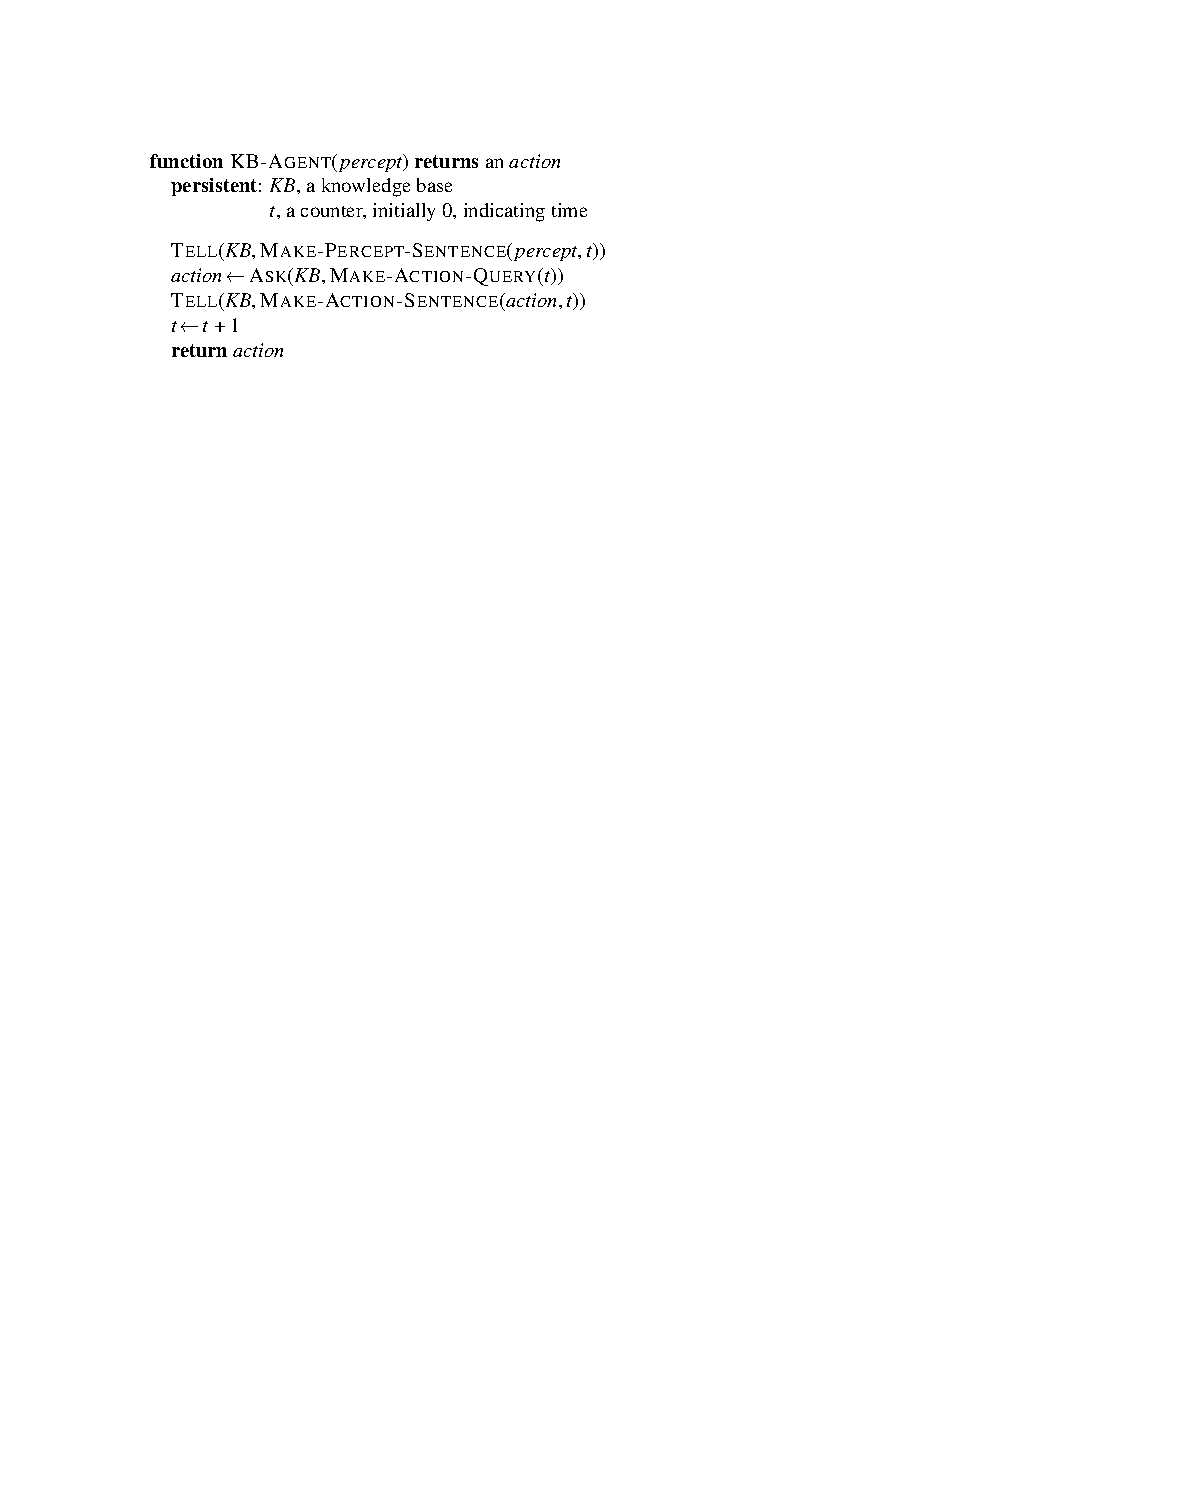
\includegraphics[alt={aima fig 07_01 kb agent},height=1in]{aima-fig-07_01-kb-agent.pdf}


\begin{itemize}
\item Logical agents are described at the \textbf{knowledge level} using \textbf{declarative} statements of knowledge and goals.
\item At the \textbf{implemetation level} we use a \textbf{procedureal} approach, encoding behaviors directly in program code.
\end{itemize}
\section{The Wumpus World}
\label{sec:org68c7cf0}





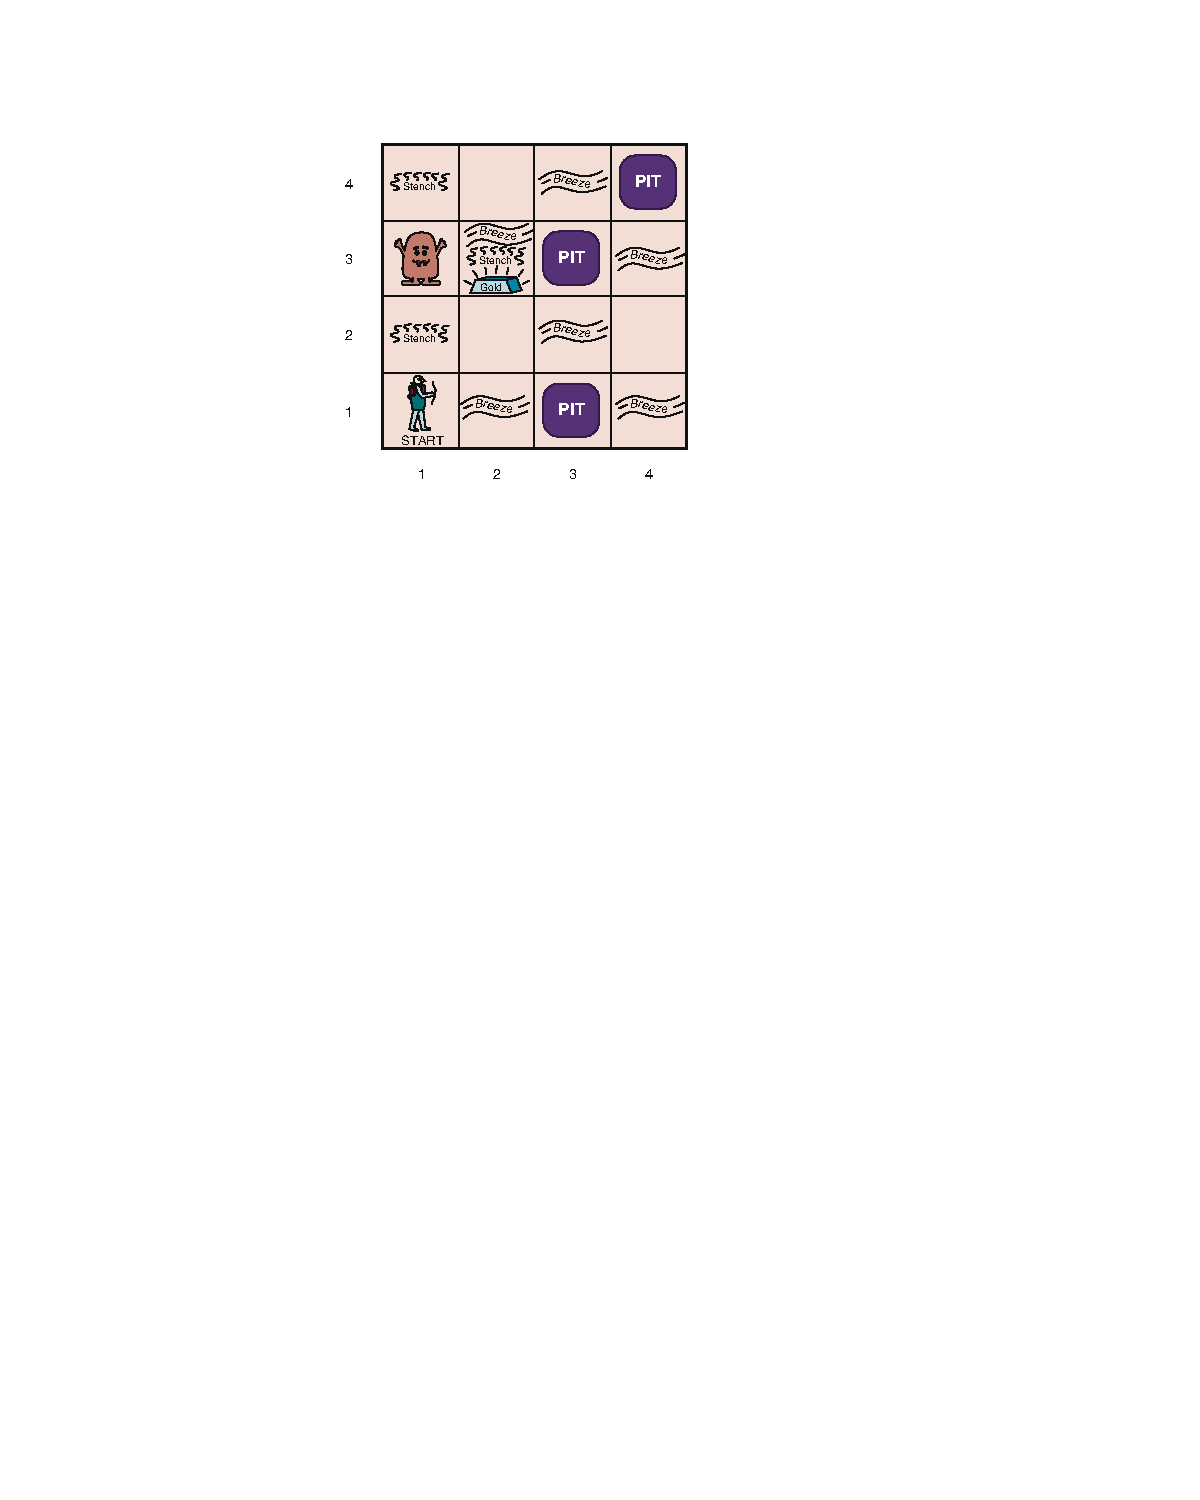
\includegraphics[alt={aima fig 07_02 wumpus world},height=1in]{aima-fig-07_02-wumpus-world.pdf}







A cave that you can drop into or climb out of at square [1, 1].

\begin{itemize}
\item \textbf{Performance measure}: +1000 for climbing out of the cave with the gold, –1000 for falling into a pit or being eaten by the wumpus, –1 for each action taken, –10 for using the arrow. The game ends either when the agent dies or when the agent climbs out of the cave.
\end{itemize}




\begin{itemize}
\item \textbf{Environment}: A 4×4 grid of rooms, agent always starts at [1,1], facing east. Gold and the wumpus placed uniformly randomly from the squares other than the start square. Each non-start square can be a pit with probability 0.2.

\item \textbf{Actuators}: Forward, TurnLeft by \(90^\circ\), or TurnRight by \(90^\circ\). The agent dies if it enters pit or a live wumpus square.  Moves into walls have no effect.  Grab picks up gold if agent in gold square. Shoot can fires arrow in direction agent is facing. The arrow continues until it either hits (and hence kills) the wumpus or hits a wall. The agent has only one arrow, so only the first Shoot action has any effect. Climb climbs out of the cave if at [1,1].
\end{itemize}
\section{First Steps Wumpus World}
\label{sec:orgb9a2fec}

\begin{itemize}
\item \textbf{Sensors}: The agent has five sensors, each of which gives a single bit of information:

\begin{itemize}
\item In squares directly (not diagonally) adjacent to wumpus, agent perceives a Stench.
\item In squares directly adjacent to a pit, the agent perceives a Breeze.
\item In the square with gold, agent perceives a Glitter.
\item When an agent walks into a wall, it perceives a Bump.
\item When the wumpus is killed, it emits a Scream perceivable anywhere in the cave.
\end{itemize}
\end{itemize}

Percepts encoded as list of five symbols indicating presense or absence (by None) of: [Stench,Breeze,Glitter,Bump,Scream] (a bit vector).



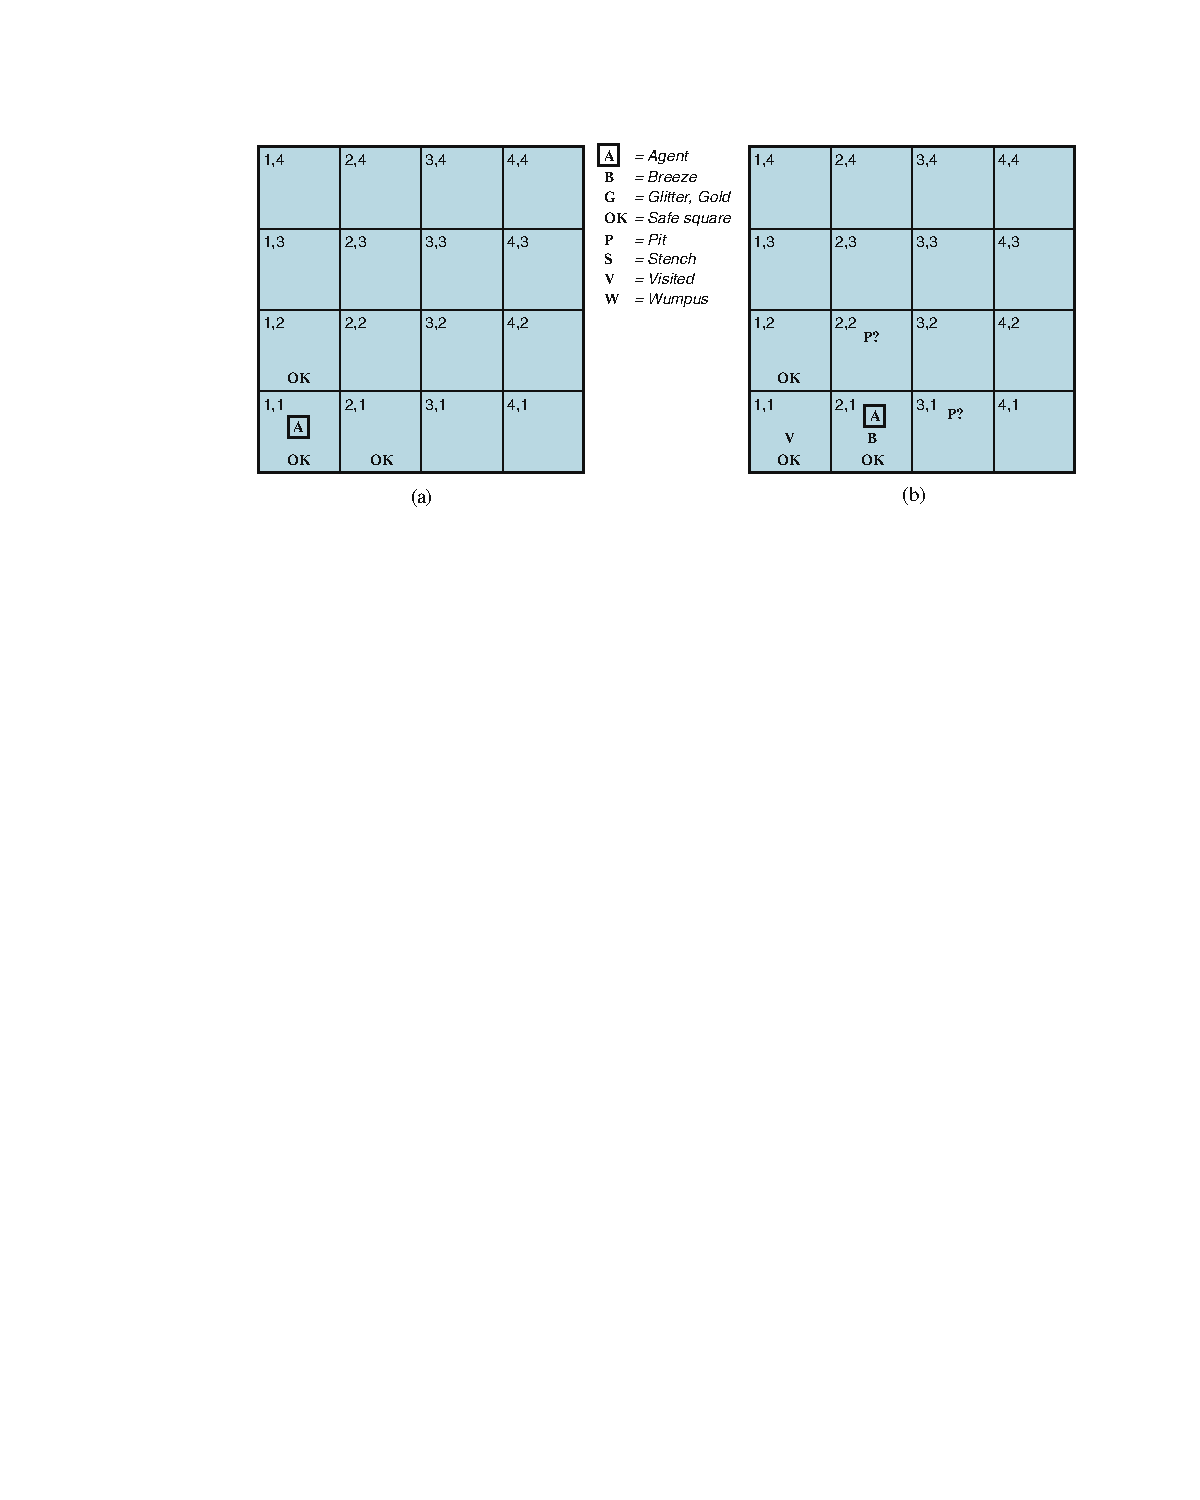
\includegraphics[alt={aima fig 07_03 first step wumpus world},height=1in]{aima-fig-07_03-first-step-wumpus-world.pdf}


\begin{itemize}
\item (a) after percept [None,None,None,None,None]
\item (b) after moving to [2,1] and perceiving [None,Breeze,None,None,None]
\end{itemize}
\section{Logic}
\label{sec:orge9bebc9}

Basics:

\begin{itemize}
\item \textbf{Syntax} specifies the form of sentences.

\begin{itemize}
\item \(x + y = 4\) is \textbf{well-formed}, but \(x4y+=\) is not.
\end{itemize}

\item \textbf{Semantics} specifies the meaning of sentences.

\begin{itemize}
\item \(x + y = 4\) is \textbf{true} in a world where \(x = 1\) and \(y = 3\).
\end{itemize}

\item \textbf{Model}: a formal specification of a \textbf{possible world}, that is, a set of assignments of values to the variables in the sentences of a knowledge base.

\begin{itemize}
\item Given a model \{\(x = 3\), \(y = 2\)\}, the sentence \(x + y = 4\) is false.
\end{itemize}
\end{itemize}

Satisfaction:

\begin{itemize}
\item "\(m\) satisfies \(\alpha\)": sentence \(\alpha\) is true in model \(m\), also "\(m\) is a model of \(\alpha\)."
\item \(M(\alpha)\) the set of all models of \(\alpha\), i.e., the set of all models in which \(\alpha\) is true.
\end{itemize}

Entailment: \(\alpha \models \beta\): \(\beta\) \textbf{follows logically} from \(\alpha\)

Formal definition of entailment:

\begin{equation*}
\alpha \models \beta \text{ if and only if } M(\alpha) \subseteq M(\beta)
\end{equation*}
\section{Possible Models of Pits in Wumpus World}
\label{sec:org7fe1a38}

The presence of pits in squares [1, 2], [2, 2] and [3, 1] gives rise to \(2^3 = 8\) possible models.


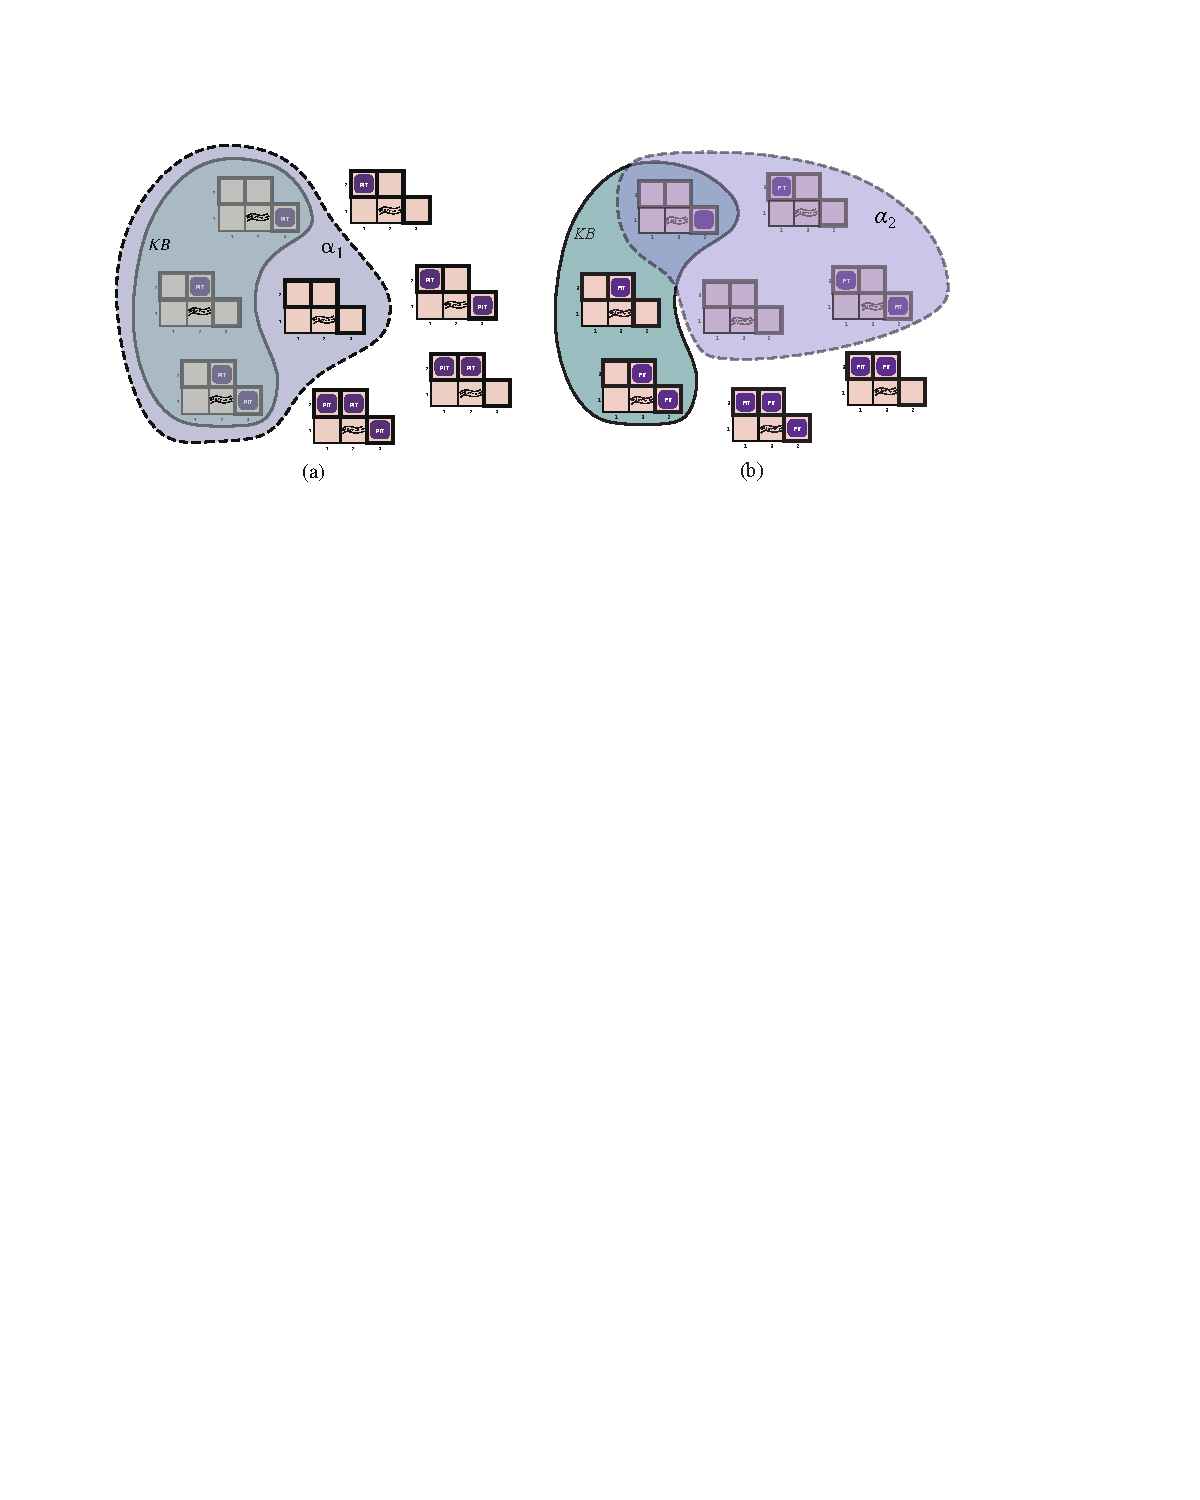
\includegraphics[alt={aima fig 07_05 possible models pits},height=1in]{aima-fig-07_05-possible-models-pits.pdf}


Solid line delineates KB based on percept [None, None, None, None, None] in [1, 1] and [None,Breeze,None,None,None] in [2, 1].

\begin{itemize}
\item (a). \(\alpha_1\) = "There is no pit in [1, 2]."  Here, \(KB \models \alpha_1\)
\item (b). \(\alpha_2\) = "There is no pit in [2, 2]."  Here, \(KB \nvDash \alpha_2\)
\end{itemize}

Logical inference via model checking: because of (b), cannot conclude \(\alpha_2\) (or \(\neg \alpha_2\)).

\begin{itemize}
\item \(M(KB) \models \alpha_1\) but  \(M(KB) \nvDash \alpha_2\)
\end{itemize}
\section{Inference Algorithms}
\label{sec:orgc9268aa}

If an inference algorithm \(i\) can derive \(\alpha\) from \(KB\), we write

\begin{equation*}
KB \vdash_i \alpha
\end{equation*}

which is pronounced "\(\alpha\) is derived from \(KB\) by \(i\)" or "\(i\) derives \(\alpha\) from \(KB\)."

\textbf{Important properties of inference algorithms}:

\begin{itemize}
\item An inference algorithm that derives only entailed sentences is called \textbf{sound} or \textbf{truth-preserving}.

\item An inference algorithm is \textbf{complete} if it can derive any sentence that is entailed.
\end{itemize}
\section{Representation vs World}
\label{sec:orgf513676}

If KB is true in the real world, then any sentence \(\alpha\) derived from KB by a sound inference procedure is also true in the real world?


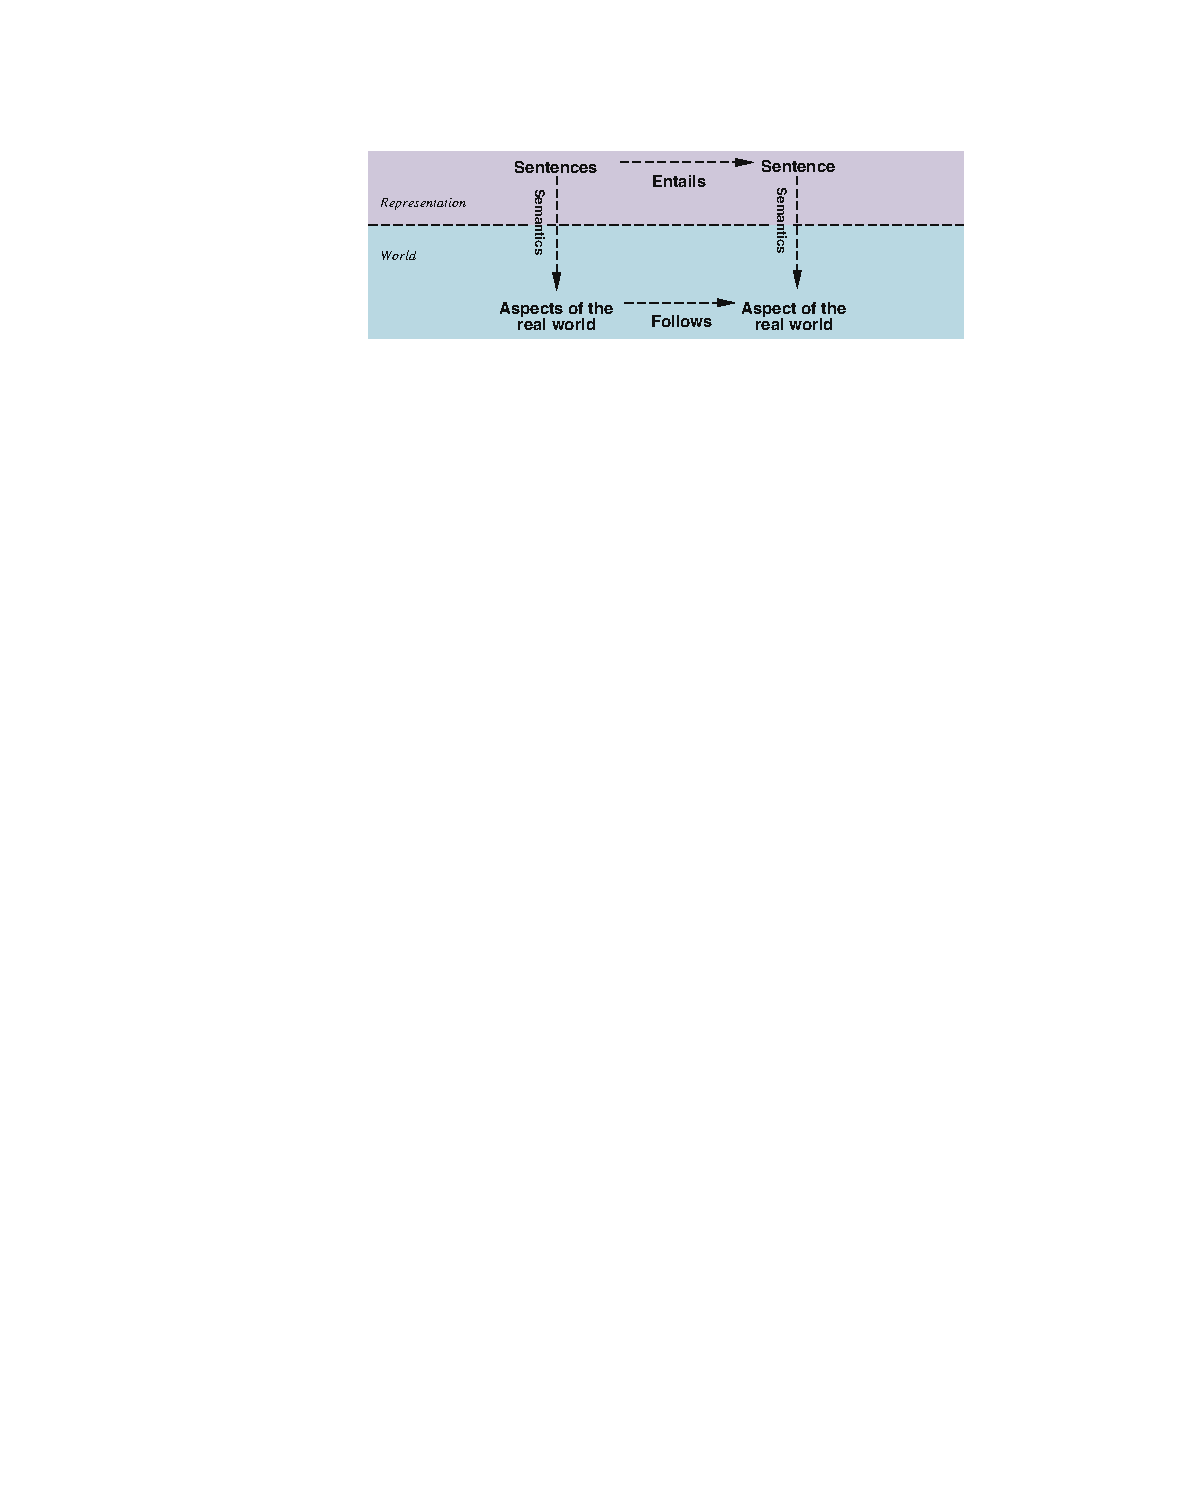
\includegraphics[alt={aima fig 07_06 representation vs world},height=1in]{aima-fig-07_06-representation-vs-world.pdf}


\textbf{Grounding}: connection between logical reasoning and the real environment.  How do we know that KB is true in the real world.

\begin{itemize}
\item Subject of volumes of philosophical investigation.
\item For us: if agent perceives it, it is true.
\end{itemize}
\section{Propositional Logic}
\label{sec:orgab154f7}

\begin{itemize}
\item \textbf{Atomic} sentences consist of a single proposition symbol.
\item Proposition symbol stands for a proposition that can be true or false.

\begin{itemize}
\item We use symbols that start with uppercase letter and may contain other letters or subscripts, e.g., : P, Q, R, \(W_{1,3}\) and FacingEast
\item True and False have fixed meanings
\end{itemize}

\item \textbf{Complex sentence}: one or more atomic sentences constructed from \textbf{logical connectives}.

\item \(\neg\) (not) Unary connective.  \(\neg W_{1,3}\) is the \textbf{negation} of \(W_{1,3}\)

\begin{itemize}
\item A \textbf{positive literal} is an atomic sentence.
\item a \textbf{negative literal} is a negated atomic sentence.
\end{itemize}

\item \(\land\) (and).  Binary connective.  \textbf{Conjunction}, e.g., \(W_{1,3} \land P_{3,1}\)

\item \(\lor\) (or).  Binary connective.  \textbf{Disjunction}, e.g., \((W_{1,3} \land P_{3,1}) \lor W_{2,2}\)

\item \(\implies\) (implies).  Binary connective.  \textbf{Implication}, e.g., \((W_{1,3} \land P_{3,1}) \implies \neg W_{2,2}\)

\begin{itemize}
\item \((W_{1,3} \land P_{3,1})\) is the \textbf{premise} or \textbf{antecedent}.
\item \(\neg W_{2,2}\) is the \textbf{conclusion} or \textbf{consequent}.
\item Also known as rules or if-then statements.
\item Some authors use \(\supset\) or \(\rightarrow\)
\end{itemize}

\item \(\iff\) (if and only if).  Binary connective. \(W_{1,3} \iff \neg W_{2,2}\) is a \textbf{biconditional}
\end{itemize}
\section{Grammar of Propositional Logic}
\label{sec:org39eddd7}


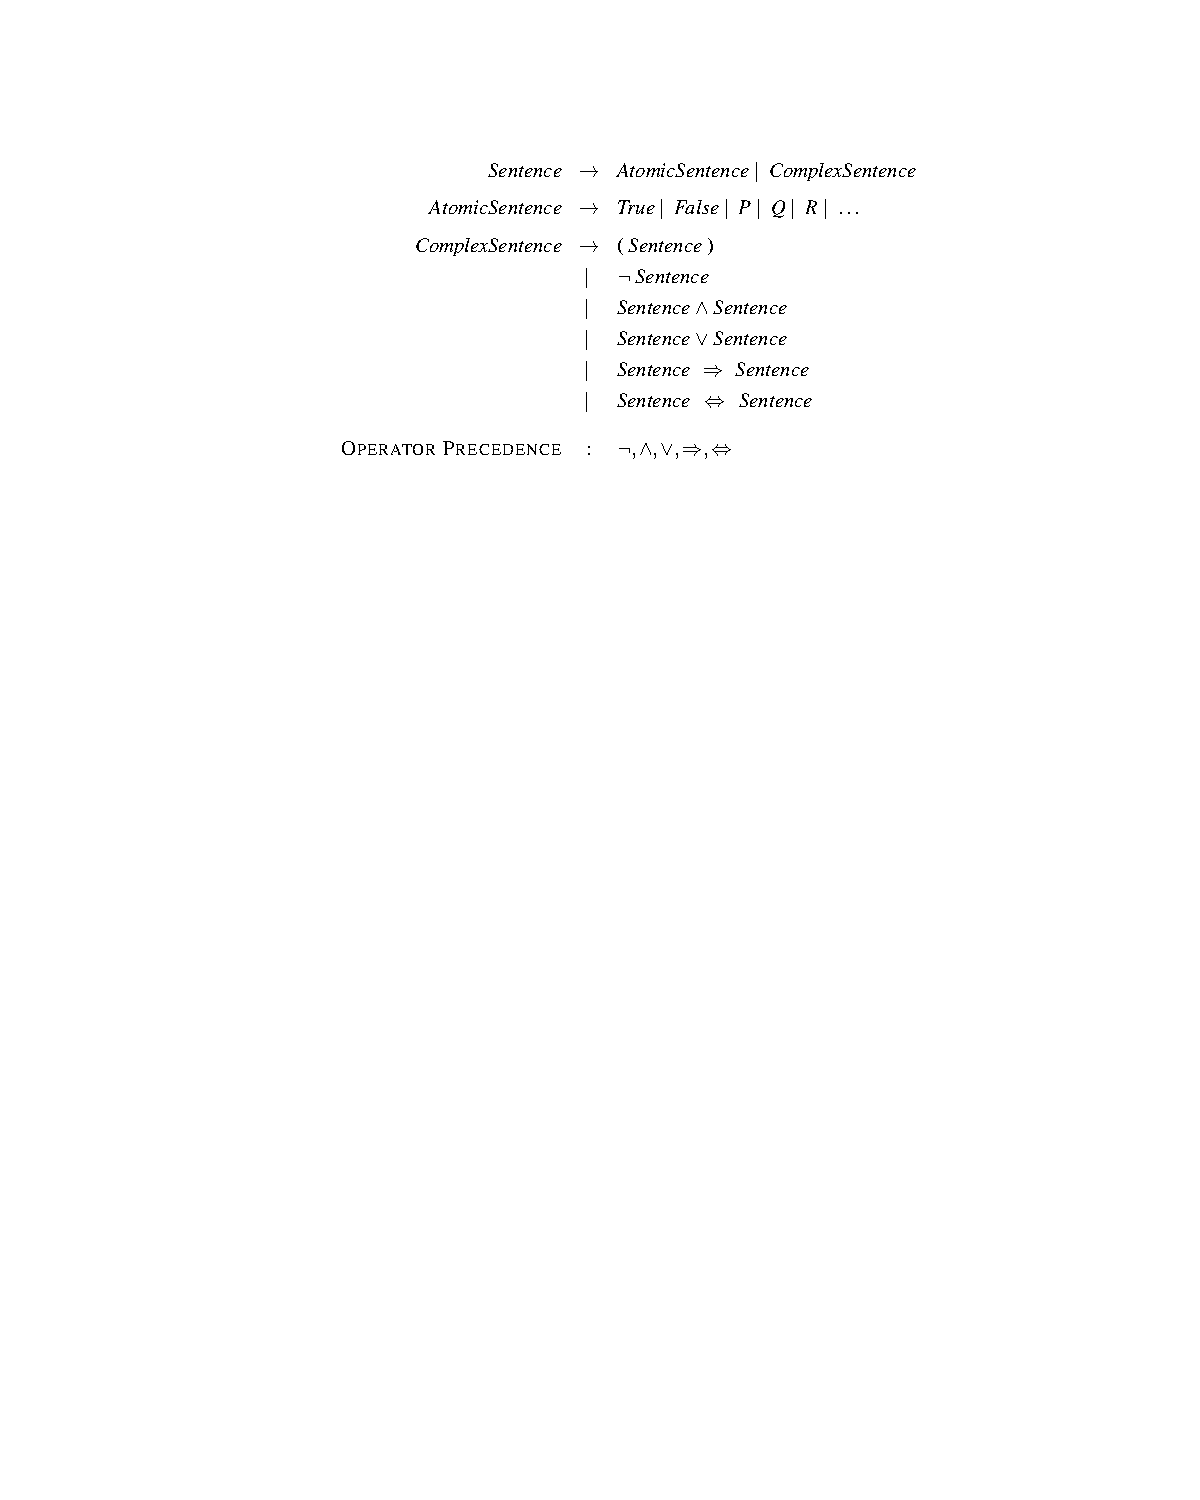
\includegraphics[alt={aima fig 07_07 grammar of popositional logic},height=1in]{aima-fig-07_07-grammar-of-popositional-logic.pdf}
\section{Semantics of Propositional Logic}
\label{sec:org1f6ea4b}


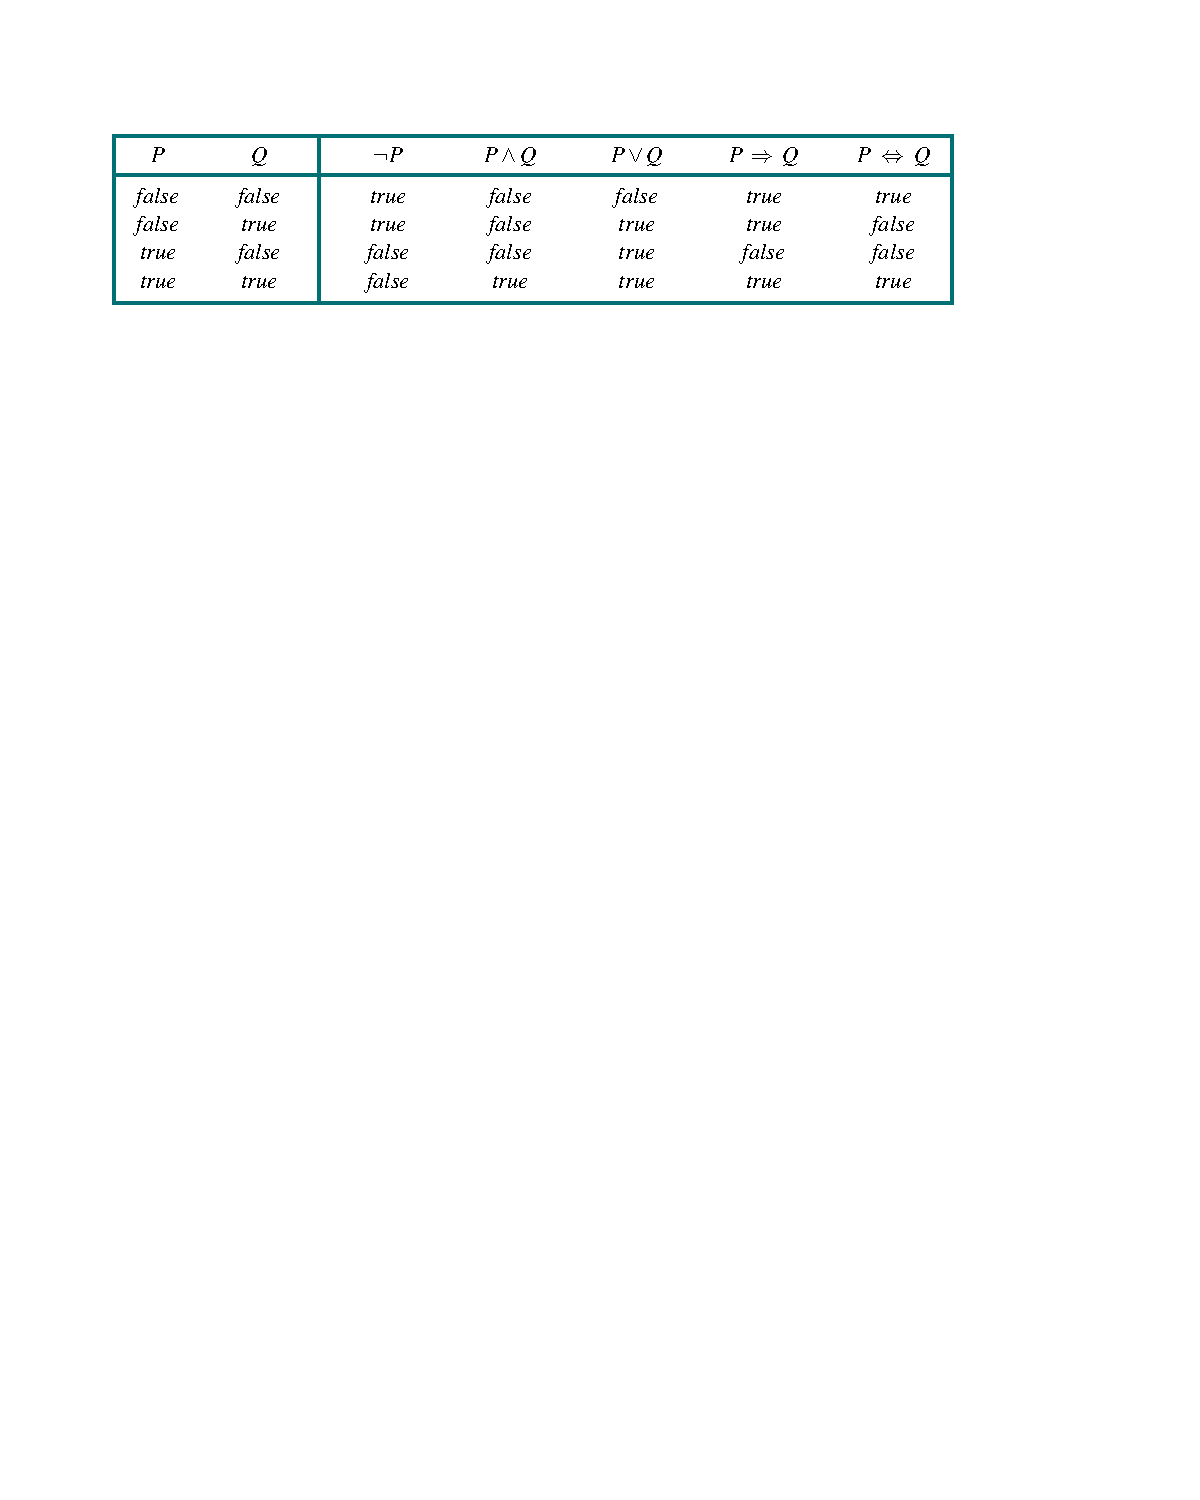
\includegraphics[alt={aima fig 07_08 truth tables logical connectives},height=1in]{aima-fig-07_08-truth-tables-logical-connectives.pdf}
\section{Propositional Theorem Proving}
\label{sec:org9b7a0b2}

So far we've done \textbf{model checking}: enumerating models and showing that the sentence must hold in all models.

Now we turn to \textbf{theorem proving}: applying rules of inference directly to the sentences in our knowledge base to construct a proof of the desired sentence without consulting models.

Some basic concepts:

\begin{itemize}
\item \textbf{Logical equivalence}: two sentences \(\alpha\) and \(\beta\) are logically equivalent if they are true in the same set of models.  \(\alpha \equiv \beta\)

\begin{itemize}
\item \(\alpha \equiv \beta\) if and only if \(\alpha \models \beta\) and \(\beta \models \alpha\)
\end{itemize}

\item \textbf{Validity}: A sentence is valid if it is true in all models. For example, the sentence \(P \land \neg P\) is valid. Valid sentences are also known as \textbf{tautologies}.

\item \textbf{Deduction theorem}: \$\text{For any sentences $\alpha$ and $\beta$ }, \(\alpha\) \models \(\beta\) \text{ if and only iff the sentence } (\(\alpha\) \implies \(\beta\)) \text{ is valid.}\$

\item A sentence is \textbf{satisfiable} if it is true in, or satisfied by, \textbf{some} model
\end{itemize}
\section{Inference Rules}
\label{sec:org7db5888}

General form:

\begin{equation*}
\frac{Givens}{Conclusions}
\end{equation*}


Modus Ponens:

\begin{equation*}
\frac{\alpha \implies \beta, \alpha}{\beta}
\end{equation*}

And-Elimination:

\begin{equation*}
\frac{\alpha \land \beta}{\alpha}
\end{equation*}
\section{Logical Equivalences}
\label{sec:org3469386}

Functionally equivalent to inference rules.  Left side on top, right side on bottom.


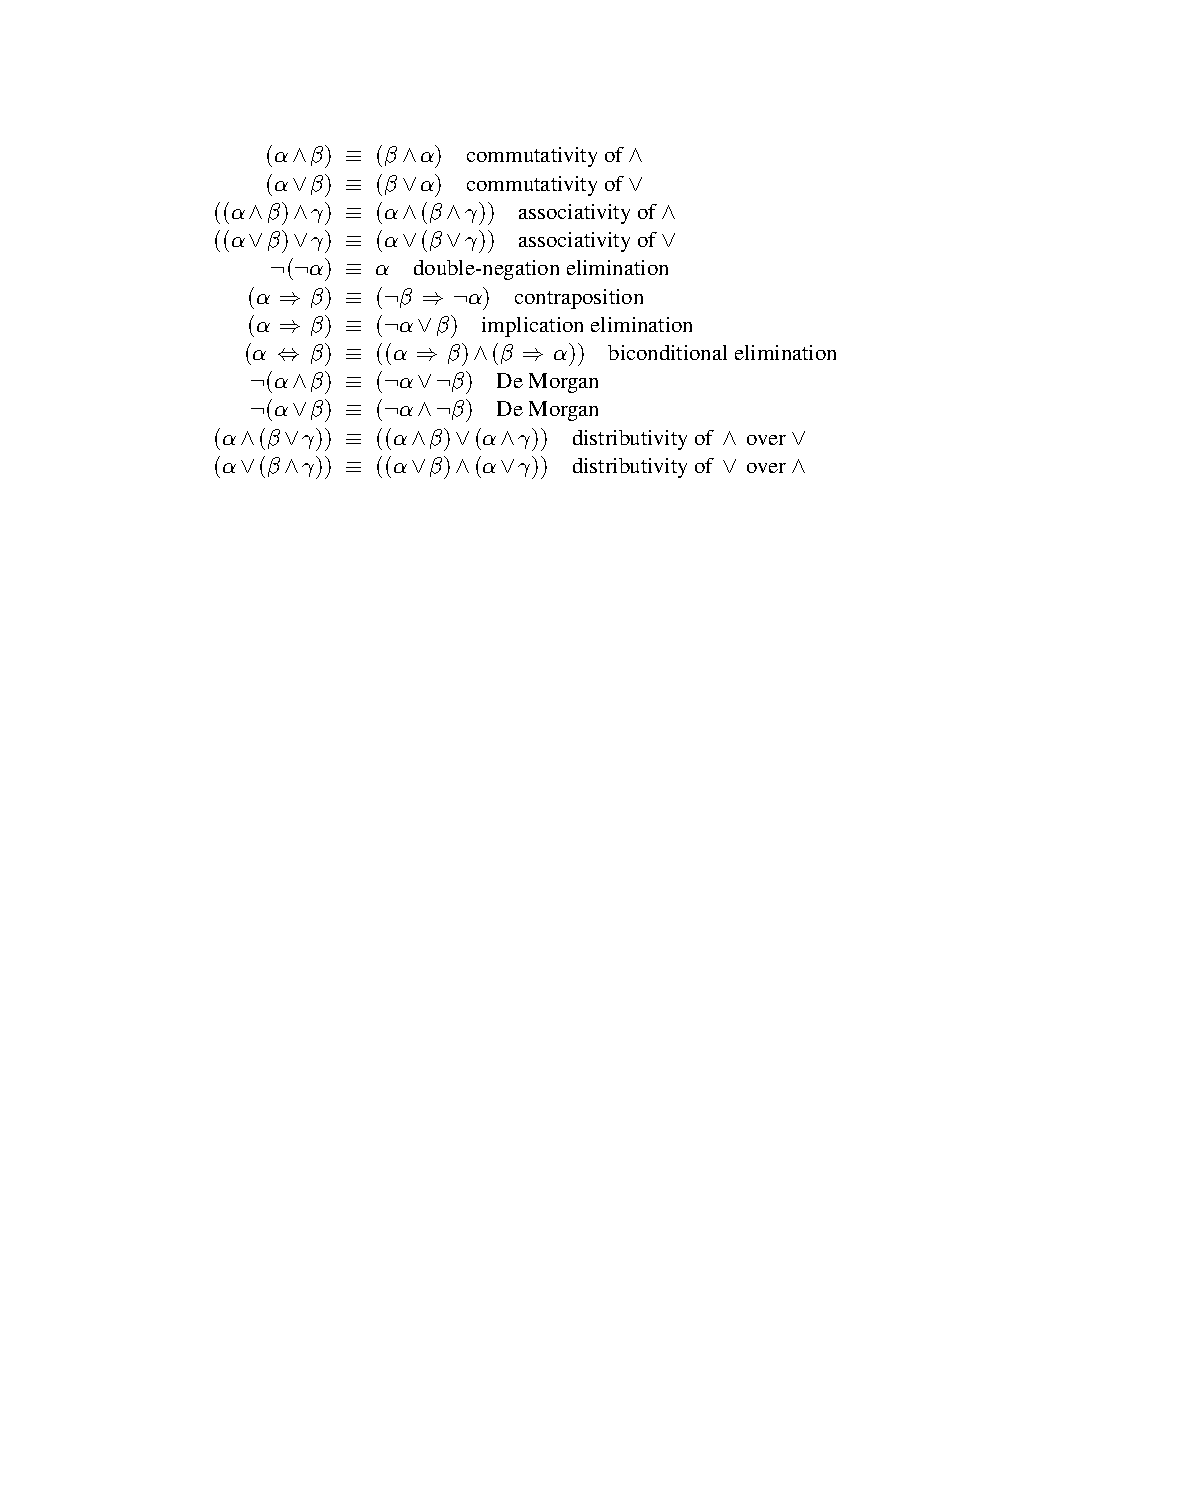
\includegraphics[alt={aima fig 07_11 logical equivalences},height=1in]{aima-fig-07_11-logical-equivalences.pdf}
\section{Representational Power of Formal Languages}
\label{sec:org416be77}

\begin{itemize}
\item Propositional logic assumes that there are facts that either hold or do not hold in the world. Each fact can be in one of two states—true or false—and each model assigns true or false to each proposition symbol.
\item First-order logic assumes that the world consists of objects with certain relations among them that do or do not hold.
\end{itemize}


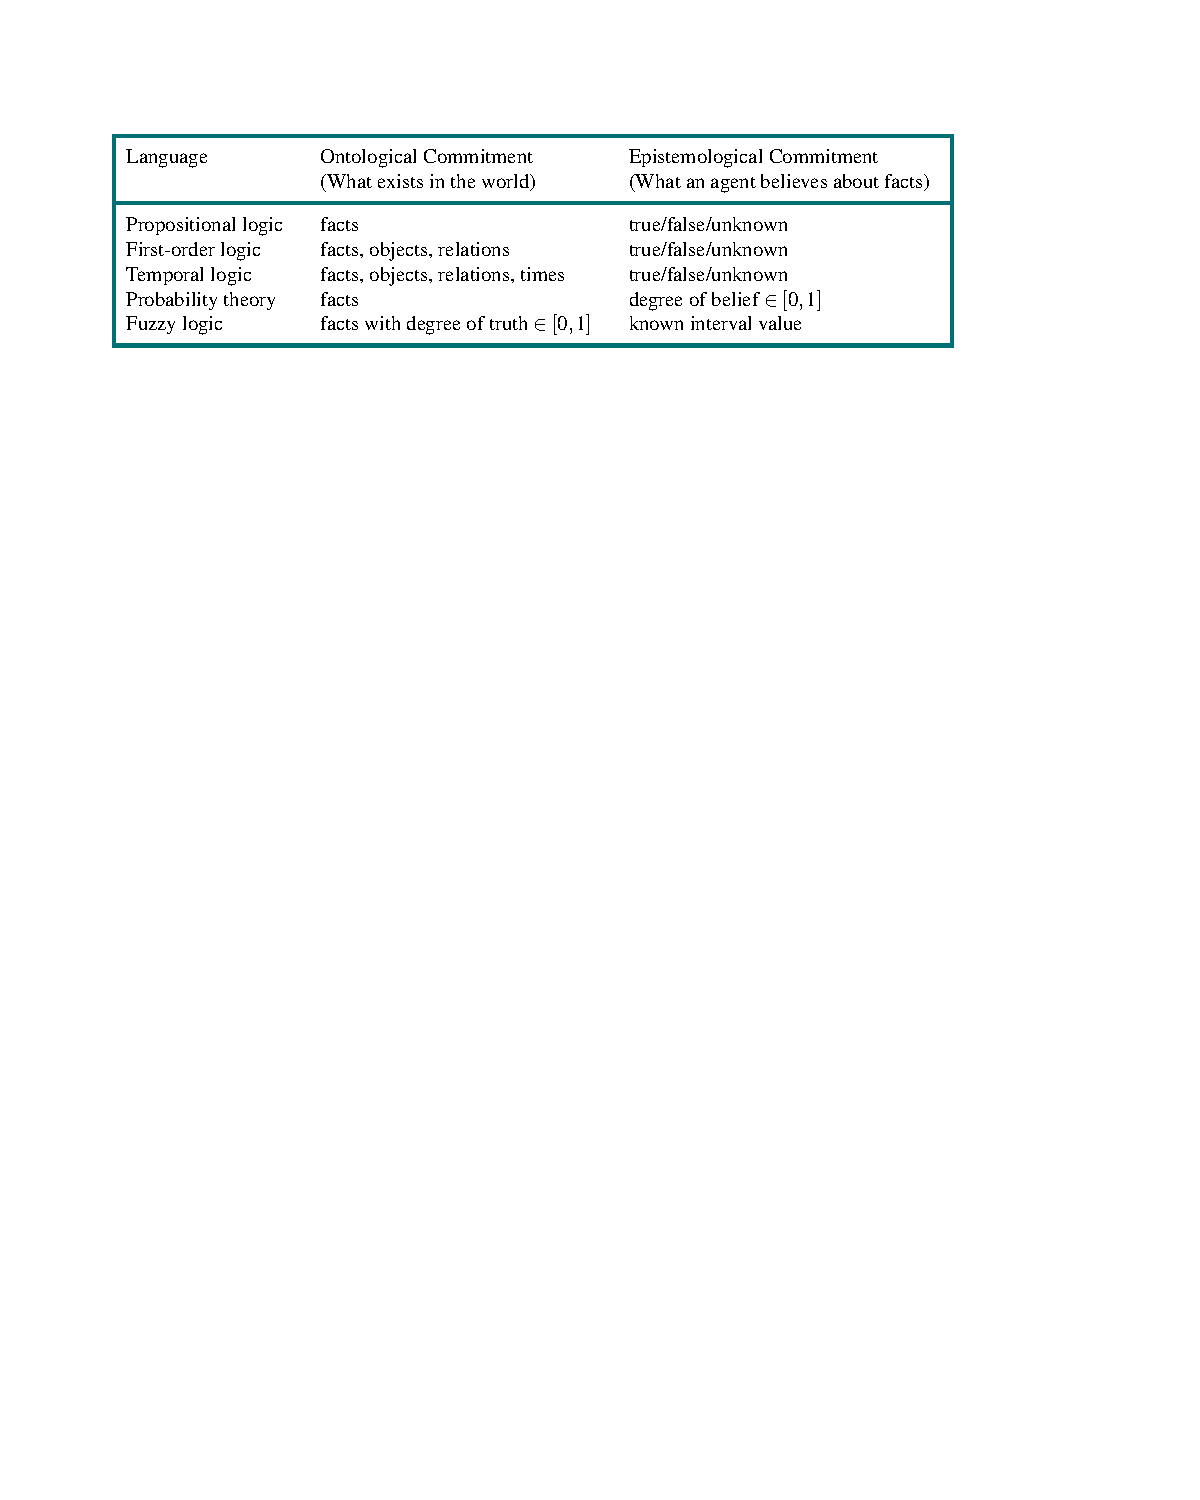
\includegraphics[alt={aima fig 08_01 ontological epistemological commitments},height=1in]{aima-fig-08_01-ontological-epistemological-commitments.pdf}


\begin{itemize}
\item \textbf{Ontological commitment}: what a language assumes about the nature of reality.
\item \textbf{Epistemological commitments}: the possible states of knowledge a language allows with respect to each fact.
\end{itemize}

\textbf{Sapir-Whorf Hypothesis}: you can only think things you can express in a language you know.
\section{Representational Power of First-Order Logic}
\label{sec:org10def66}


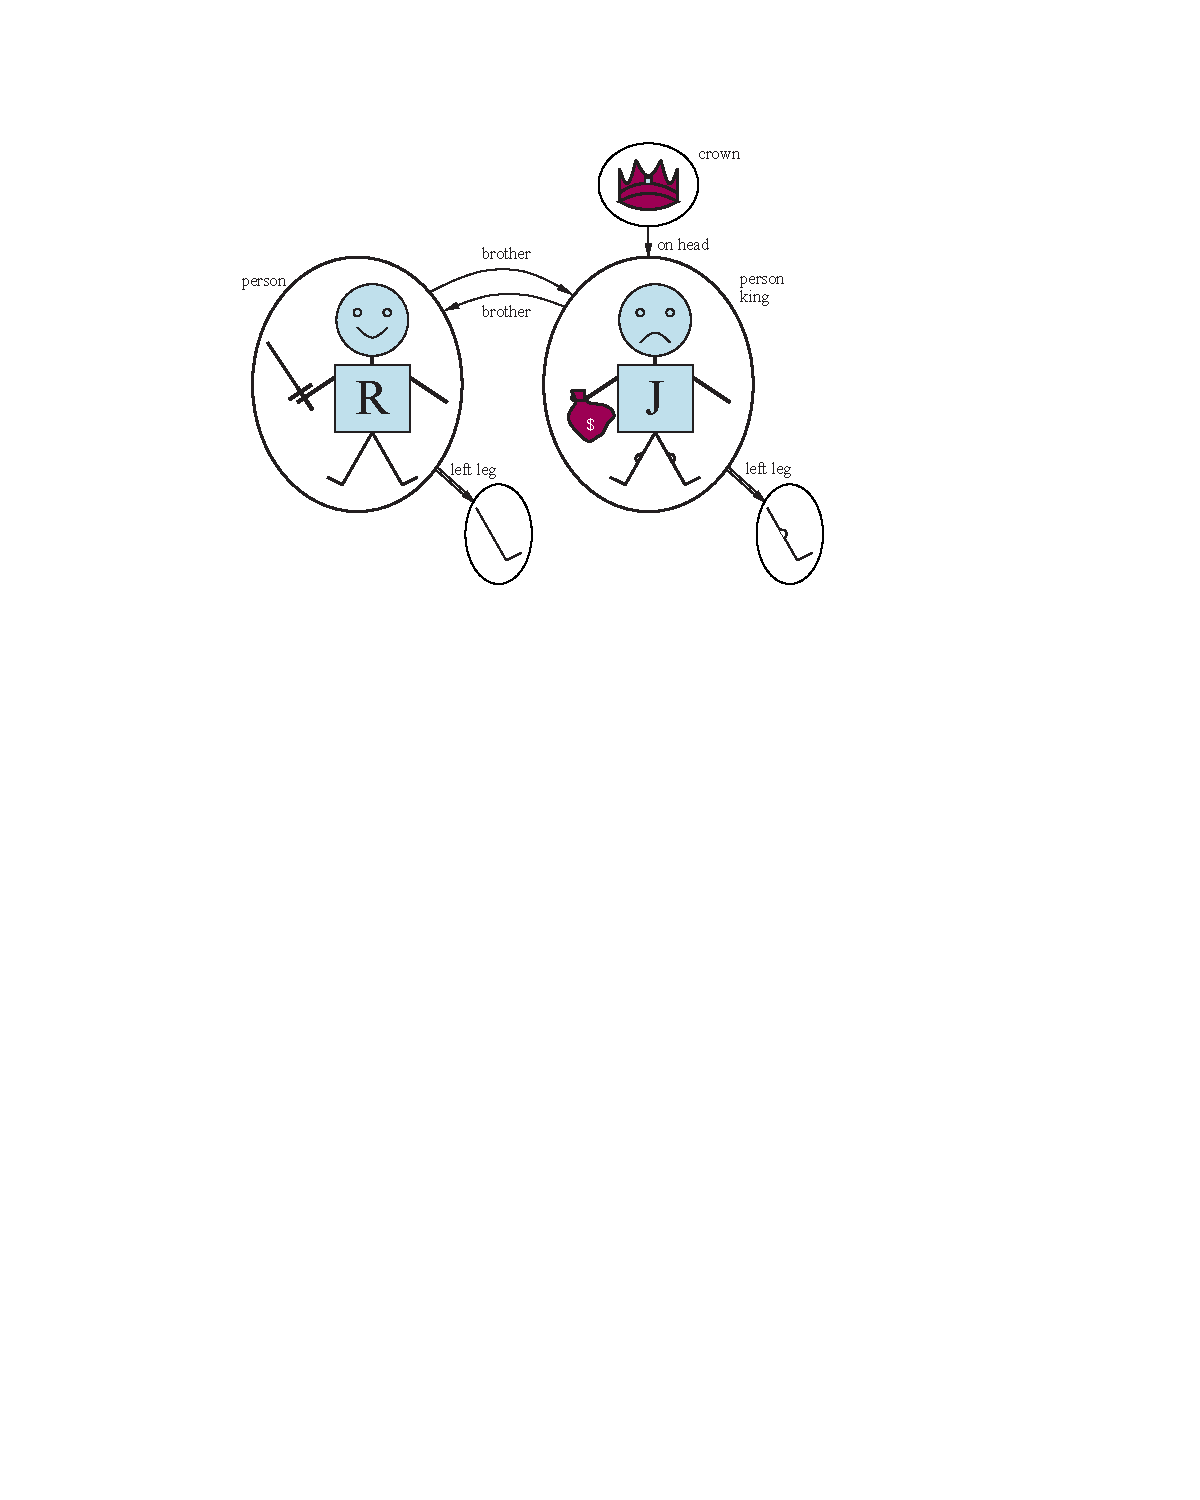
\includegraphics[alt={aima fig 08_02 person king model},height=1in]{aima-fig-08_02-person-king-model.pdf}
\section{First-Order Logic}
\label{sec:orgb440964}

Also known as first-order predicate logic.

\begin{itemize}
\item \textbf{Constant symbols} stand for objects, e.g., \(Richard\), \(John\).

\item \textbf{Predicate symbols} stand for relations, e.g., \(Brother(Richard, John)\).

\item \textbf{Function symbols} stand for functions, e.g., \(LeftLeg(John)\)

\begin{itemize}
\item Above is also a \textbf{term} -- a logical expression that refers to an object.
\end{itemize}
\end{itemize}

Atomic sentences:

\begin{itemize}
\item \(Brother(Richard, John)\), \(Married(Father(Richard),Mother(John))\)
\end{itemize}

Complex sentences:

\begin{itemize}
\item \(Brother(Richard,John) \land Brother(John,Richard)\)
\end{itemize}

Quantifiers:

\begin{itemize}
\item \(\forall x, King(x) \implies Person(x)\)

\begin{itemize}
\item For all objects \(x\), if \(x\) is a \(King\), then \(x\) is a \(Person\).
\item In English:"All kings are persons."
\end{itemize}
\item \(\exists x, Crown(x) \land Onhead(x, John)\)

\begin{itemize}
\item There exists an \(x\) such that \(x\) is a \(Crown\) and \(x\) is on the head of \(John\).
\item In English: "John has a crown on his head."
\end{itemize}
\end{itemize}
\section{Knowledge Representation}
\label{sec:orgaa767d4}

Complex reasoning requires representation of abstract concepts:

\begin{itemize}
\item Events
\item Time
\item Physical Objects
\item Beliefs
\end{itemize}

Representing abstract concepts is sometimes called \textbf{ontological engineering}.
\section{Physical Objects}
\label{sec:org6ab9c6b}

\begin{itemize}
\item Categories vs objects

\begin{itemize}
\item A category is a set which represents some commonality among objects in the set.
\item Individuation: division into distinct objects
\end{itemize}

\item Part vs whole

\begin{itemize}
\item Composites represent structural relationships between parts
\item \(Biped(a) \implies \exists l_1, l_2, b, Leg(l_1) \land Leg(l_2) \land Body(b) \land PartOf(l_1, b) \dots\)
\end{itemize}

\item Measures

\begin{itemize}
\item Kind of quantity, e.g., length, weight, mass
\item Units, conversions
\end{itemize}

\item Count nouns vs mass nouns

\begin{itemize}
\item Count noun: 2 glass*es* of water -- 1 glass is \textbf{FEWER} than 2 glasses

\item Mass noun: a gallon of water -- 1 gallon is \textbf{LESS THAN} 2 gallons
\end{itemize}

\item Intrinsic vs extrinsic properties

\begin{itemize}
\item Intrinsic properties part of essence of object
\item Extrinsic properties are not retained under subdivision
\item Gold still glitters when split into two equal parts, but each part now has half the mass, weight.
\end{itemize}
\end{itemize}
\section{Categories and Objects}
\label{sec:org423a3fd}

Two choices for representing a category:

\begin{itemize}
\item use \textbf{predicates}, like \(Basketball(b)\), or
\item \textbf{reify} the category as an object itself and say

\begin{itemize}
\item \(Member(b,Basketballs)\) or \(b \in Basketballs\).
\end{itemize}
\end{itemize}

Can also have subcategories, e.g., \(Subset(Basketballs,Balls)\) or \(Basketballs \subset Balls\).

Categories organize knowledge into \textbf{inheritance hierarchies}, or \textbf{taxonomies}, like this upper ontology of the world:


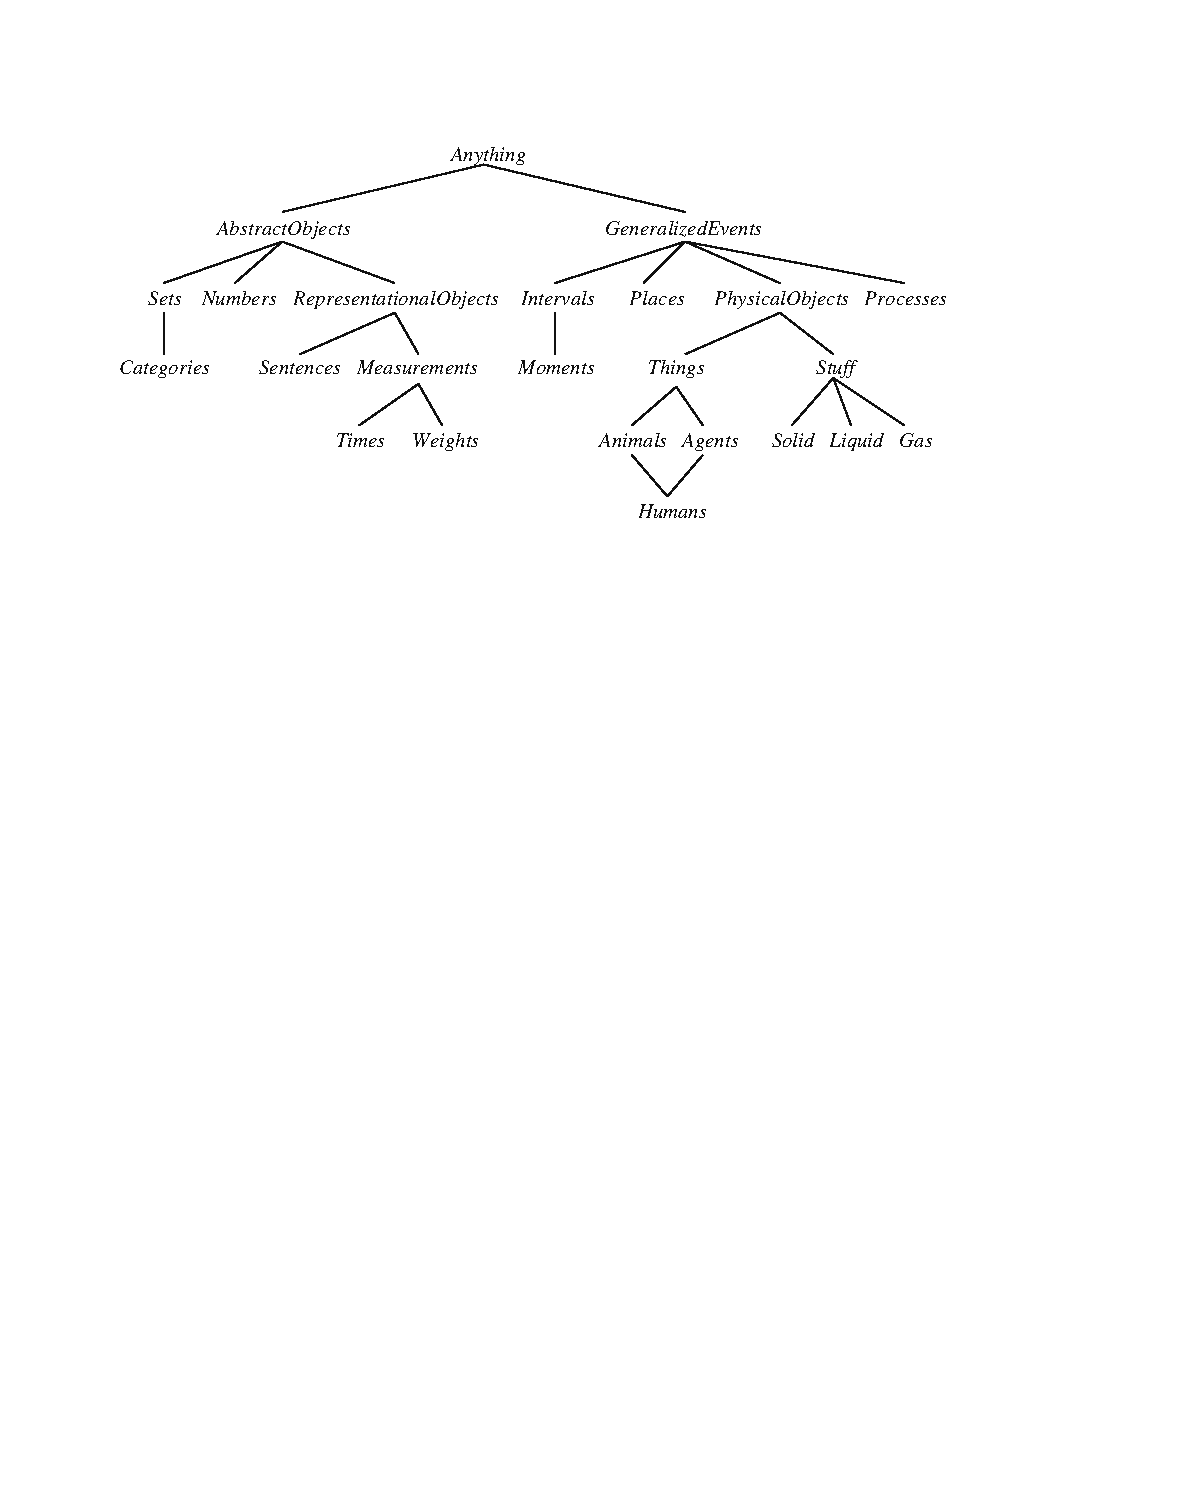
\includegraphics[alt={aima fig 10_01 upper ontology world},height=1in]{aima-fig-10_01-upper-ontology-world.pdf}
\section{Events and Time}
\label{sec:orgef0f330}

An \textbf{event calculus} encodes events, fluents, and time points, and the relationships between them.

\begin{itemize}
\item A \textbf{fluent} is an aspect of the world that changes, an object that changes over time.
\item An \textbf{event} is a temporal, locational, or relational fixing of object(s).

\begin{itemize}
\item \(E_1 \in Flyings \land Flyer(E_1,Shankar) \land Origin(E_1,SF) \land Destination(E_1,DC)\)
\end{itemize}

\item A \textbf{time predicate}, \(T\), fixes a fluent or event in time, e.g.,

\begin{itemize}
\item \(T(f, t_1, t_2)\) Fluent \(f\) is true for all times between \(t_1\) and \(t_2\)
\item \(Happens(e,t1,t2)\) Event \(e\) starts at time \(t_1\) and ends at \(t_2\)
\end{itemize}
\end{itemize}


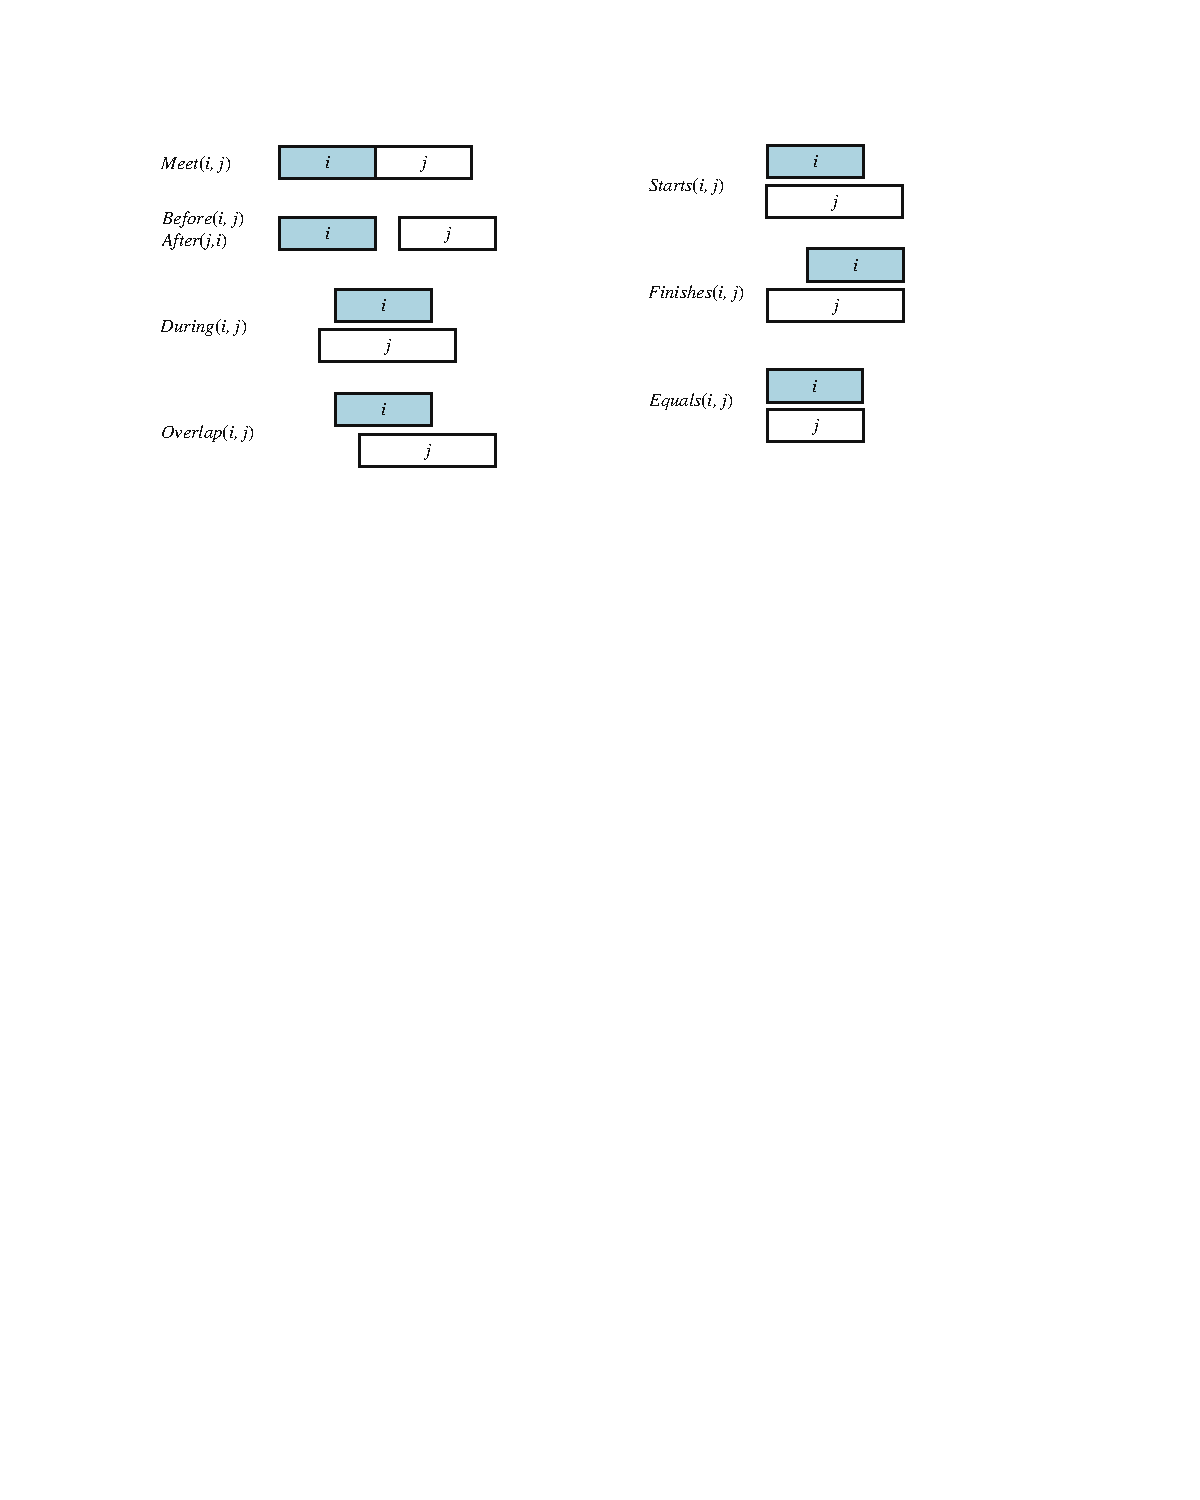
\includegraphics[alt={aima fig 10_02 predicates time intervals},height=1in]{aima-fig-10_02-predicates-time-intervals.pdf}
Predicates on time intervals.
\section{Fluents}
\label{sec:org2ed4b19}


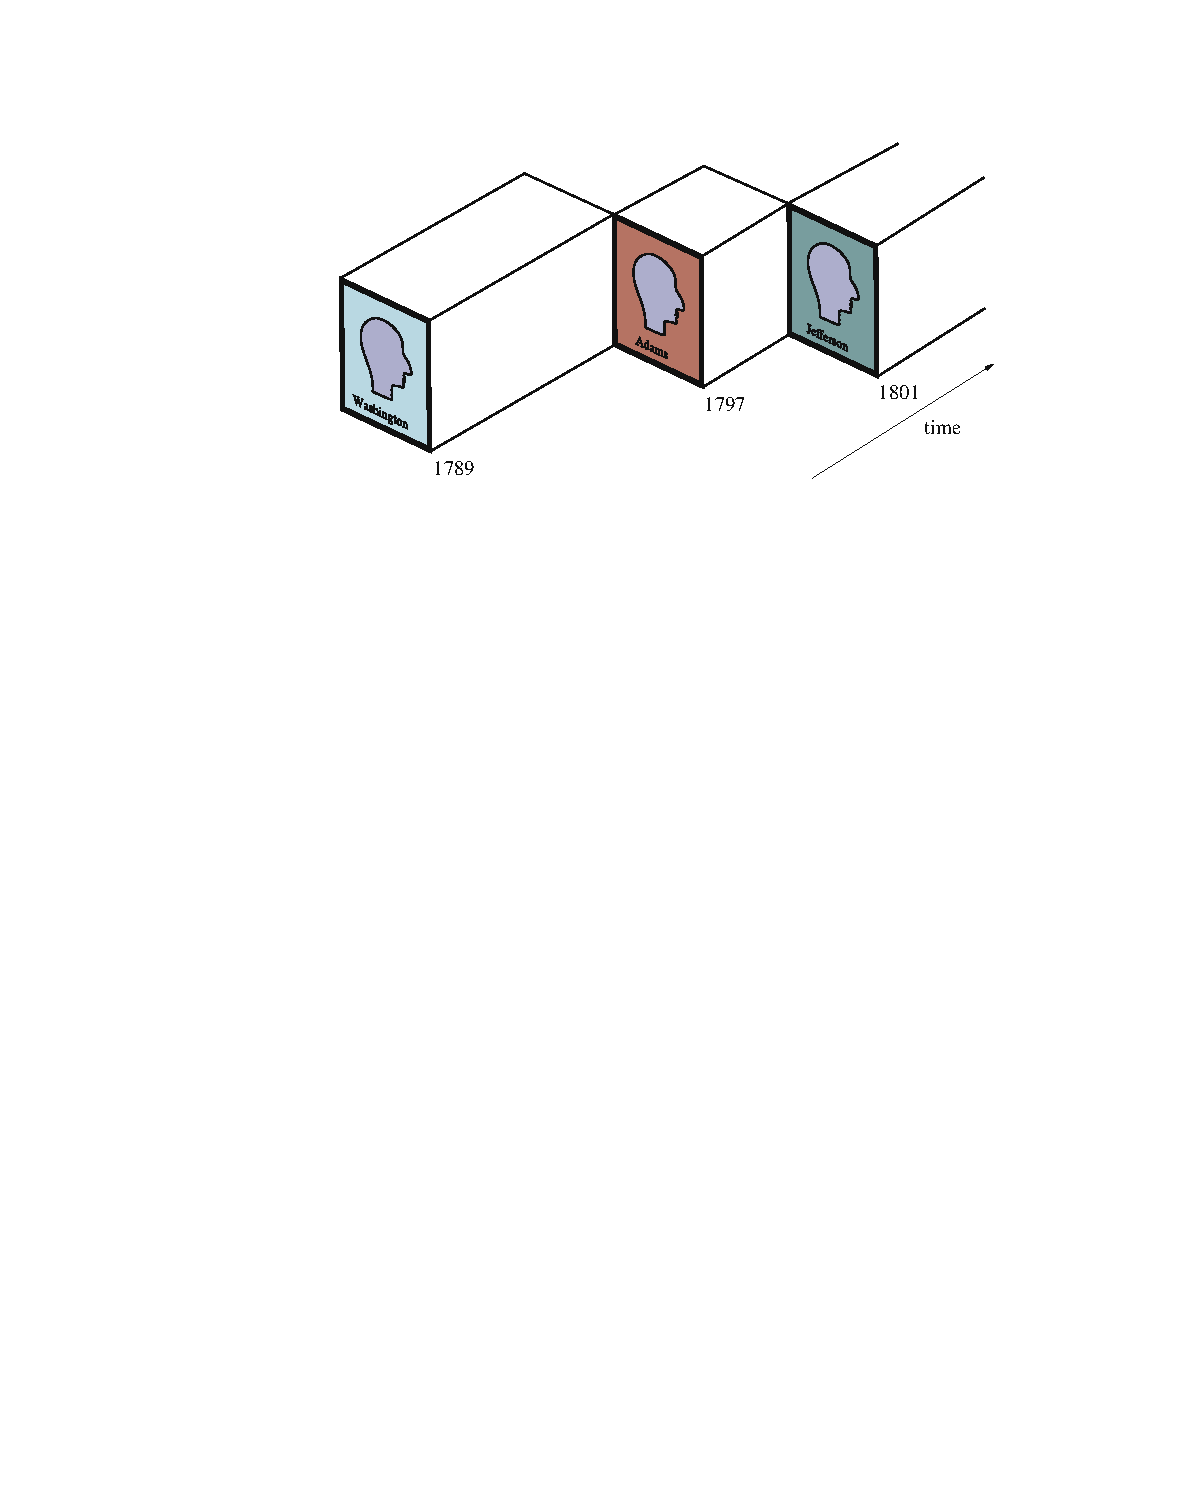
\includegraphics[alt={aima fig 10_03 schematic object president},height=1in]{aima-fig-10_03-schematic-object-president.pdf}


\$
T(Equals(President(USA),GeorgeWashington),Begin(AD1789),End(AD1797))
\begin{equation*}

Use $Equals$ function instead of logical predicate $=$ because can't have have predicate as argument to $T$.


## Beliefs and Attitudes


Beliefs are mental objects. Consider

\end{equation*}
Knows(Lois,CanFly(Superman))
\begin{equation*}

What if Lois knows that Clark Kent is Superman?

```{=latex}
\begin{align*}
& (Superman = Clark) \land Knows(Lois,CanFly(Superman)) \\
& \hspace{.2in} \models Knows(Lois,CanFly(Clark))
\end{align*}
```

This gets out of hand quickly.  Need **modal logic**, which includes modal operators that take sentences as arguments instead of terms.  $A$ knows $P$ becomes:

\end{equation*}
\bm{K}\textsubscript{A} P
\begin{equation*}

Where \(\bm{K}\) is the modal operator for knowledge.  First argument \(A\) is the agent and written as subscript.  Second argument, \(P\), is the proposition that \(A\) "knows."

\#\# Semantic Networks

Originally called \textbf{\textbf{existential graphs}}.

```\{=latex\}
\begin{center}
```
![](aima-fig-10_04-semantic-network-4-objects.pdf){height="60%"}
```{=latex}
\end{center}
```

\#\# Closing Thoughts

\begin{itemize}
\item \textbf{\textbf{Much}} more to knowledge-based AI than presented here
\item This overview enough to feel confident discussing knowledge-based AI at cocktail parties
\item Knowledge-based AI heart of \textbf{expert systems}, failure of which led to an AI winter

\begin{itemize}
\item Knowledge-acquisition bottleneck hindered completeness

\begin{itemize}
\item Practically impossible for a physician to encode his/her medical knowledge in rules.
\end{itemize}

\item Knowledge AI fell out of favor, has never really recovered the mantle of AI

\begin{itemize}
\item Didn't stop Doug Lennat and his team at [Cycorp](\url{https://cyc.com/}) from trying.
\end{itemize}
\end{itemize}
\end{itemize}
\end{document}
